\documentclass[xetex,mathserif,serif]{beamer}
\usepackage{polyglossia}
\setdefaultlanguage[babelshorthands=true]{english}
\usepackage{minted}
\usepackage{tabu}
\usepackage{graphicx}

\useoutertheme{infolines}

\usepackage{fontspec}
\setmainfont{FreeSans}
\newfontfamily{\russianfonttt}{FreeSans}

\definecolor{links}{HTML}{2A1B81}
\hypersetup{colorlinks,linkcolor=,urlcolor=links}

\setbeamertemplate{blocks}[rounded][shadow=false]
\setbeamercolor*{block title alerted}{fg=red!50!black,bg=red!20}
\setbeamercolor*{block body alerted}{fg=black,bg=red!10}

\tabulinesep=0.8mm

\title{Siamese Neural Networks for One-shot Image Recognition}
\author{Alexander Smirnov}
\date{12.11.2019}

\begin{document}

	\frame{\titlepage}

	\begin{frame}
		\frametitle{Problem}
			\begin{itemize}
		 		\item Learning good features computationally expensive
		 		\item Little data is available
			\end{itemize}
	\end{frame}
	
	\begin{frame}
		\frametitle{Solution overview}
			\begin{itemize}
		 		\item Siamese neural networks structure to rank similarity between inputs
		 		\item Once a network has been tuned it may be applied not just to predict on new data but to entirely new classes
                \item Correctly making predictions given only a single example of each new class
			\end{itemize}
	\end{frame}
	
	\begin{frame}
		\frametitle{Example}
    		\begin{figure}[h]
                \center{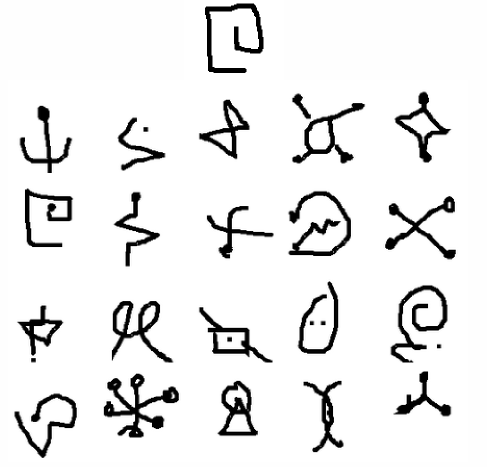
\includegraphics[scale=0.25]{images/example.png}}
                \caption{Example of a 20-way one-shot classification task using the Omniglot dataset. The lone test image is shown above the grid of 20 images representing the possible unseen classes that we can choose for the test image. These 20 images are our only known examples of each of those classes}
                \label{fig:image}
            \end{figure}
	\end{frame}			
	
	\begin{frame}
		\frametitle{Plan}
    		 \begin{figure}[h]
                \center{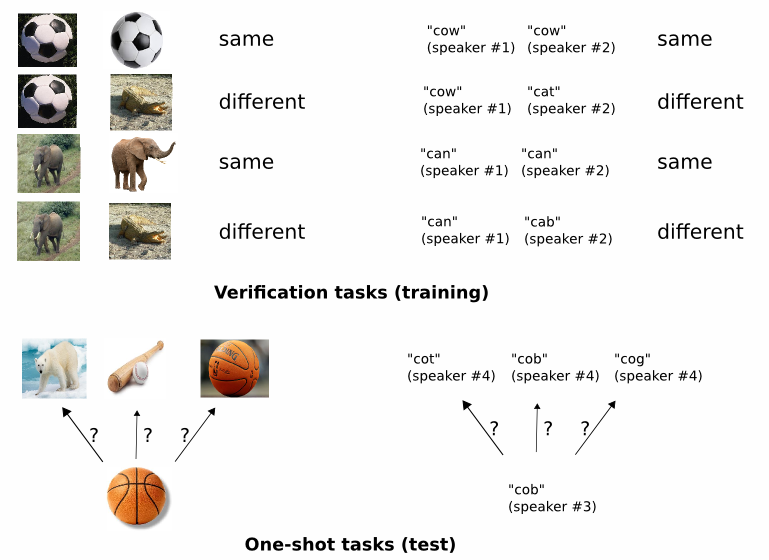
\includegraphics[scale=0.18]{images/strategy.png}}
                \caption{General strategy.}
                \label{fig:image}
            \end{figure}
			\begin{enumerate}
		 		\item Train a model to discriminate between a collection of same/different pairs
				\item Generalize to evaluate new categories based on learned feature mappings for verification
			\end{enumerate}
	\end{frame}
	
	\begin{frame}
		\frametitle{Approach}
			\begin{itemize}
				\item Learn a neural network that can discriminate between the class-identity of image pairs (verification task)
				\item The verification model learns to identify input pairs according to the probability that they belong to the same class or different classes
				\item This model can then be used to evaluate new images, exactly one per novel class, in a pairwise manner against the test image
				\item The pairing with the highest score according to the verification network is then awarded the highest probability for the one-shot task
			\end{itemize}
	\end{frame}
	
	\begin{frame}
		\frametitle{Model}
    		\begin{figure}[h]
                \center{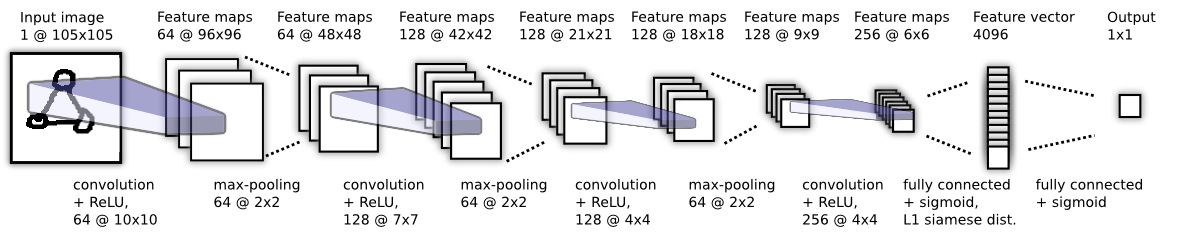
\includegraphics[scale=0.22]{images/model.png}}
                \caption{Best convolutional architecture selected for verification task. Siamese twin joins immediately after the 4096 unit layer where the L1 component-wise distance between vectors is computed}
                \label{fig:image}
            \end{figure}
	\end{frame}	
	
	\begin{frame}
		\frametitle{Learning}
			\begin{itemize}
		 		\item Loss function
        			\begin{itemize}
        		 		\item Regularized cross-entropy
        			\end{itemize}
        		\item Weight initialization
        			\begin{itemize}
        		 		\item Weights in the convolutional layers initialized from a normal distribution with zero-mean and a standard deviation of $10^{-2}$
        		 		\item Biases were also initialized from a normal distribution, but with mean $0.5$ and standard deviation $10^{-2}$
        			\end{itemize}
        		\item Schedule
        			\begin{itemize}
        		 		\item $20000$ iterations
        		 		\item $20$ — support set quantity
        		 		\item $30$ — number of validations
        			\end{itemize}
			\end{itemize}
	\end{frame}	
	
	\begin{frame}
		\frametitle{The Omniglot Dataset}
    		\begin{figure}[h]
                \center{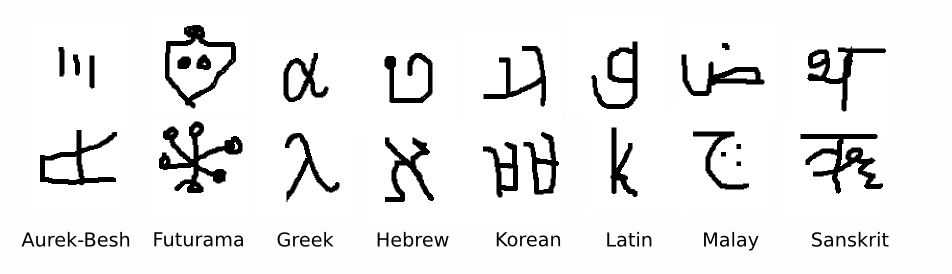
\includegraphics[scale=0.22]{images/omniglot.png}}
                \caption{The Omniglot dataset contains a variety of different images from alphabets across the world.}
                \label{fig:image}
            \end{figure}
            
            \begin{itemize}
		 		\item The number of letters in each alphabet varies considerably from about 15 to upwards of 40 characters
		 		\item All characters across these alphabets are produced a single time by each of 20 drawers
		 		\item Splitting the data into a 30 alphabet training set and a 20 alphabet evaluation set
			\end{itemize}
	\end{frame}		
	
	\begin{frame}
		\frametitle{Training}
            \begin{columns}
                \column{1\textwidth}
                    \begin{minipage}[c][0.4\textheight][c]{\linewidth}
                        \centering
                        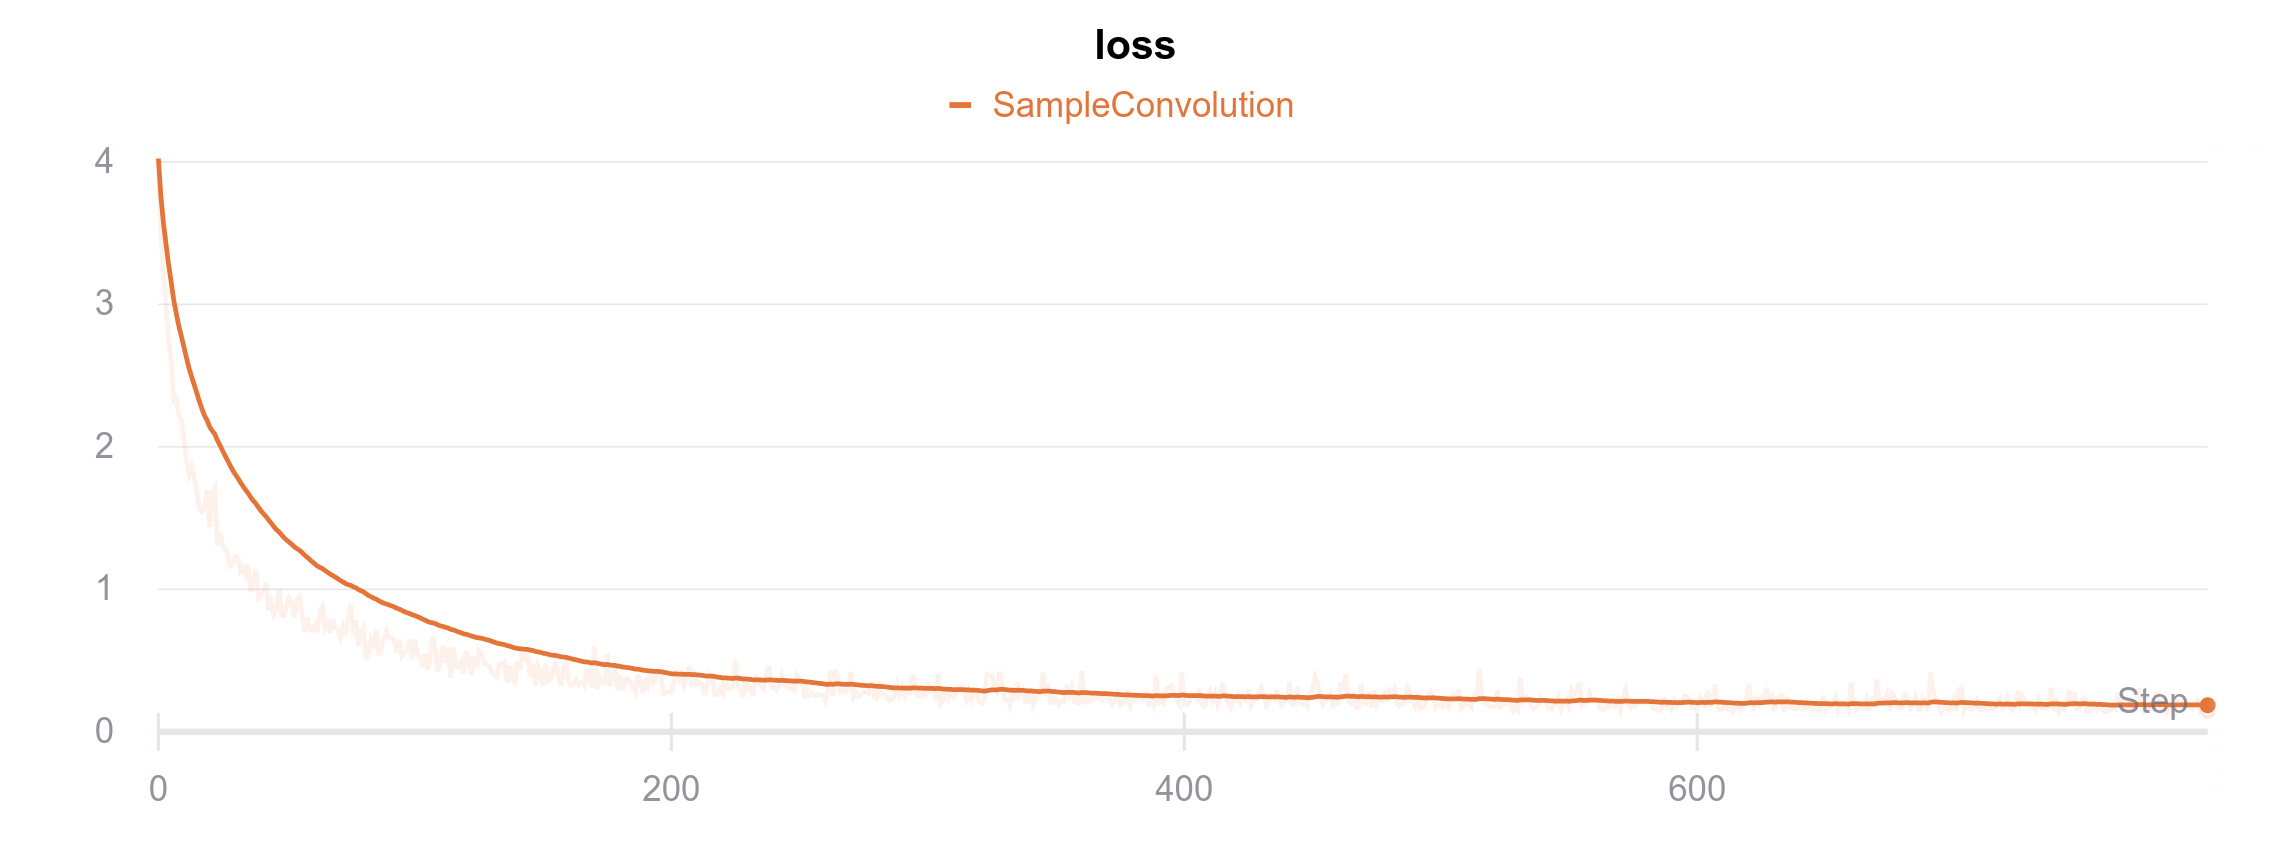
\includegraphics[width=0.7\linewidth]{images/loss.png}
                    \end{minipage}
            
                    \begin{minipage}[c][0.6\textheight][c]{\linewidth}
                        \centering
                        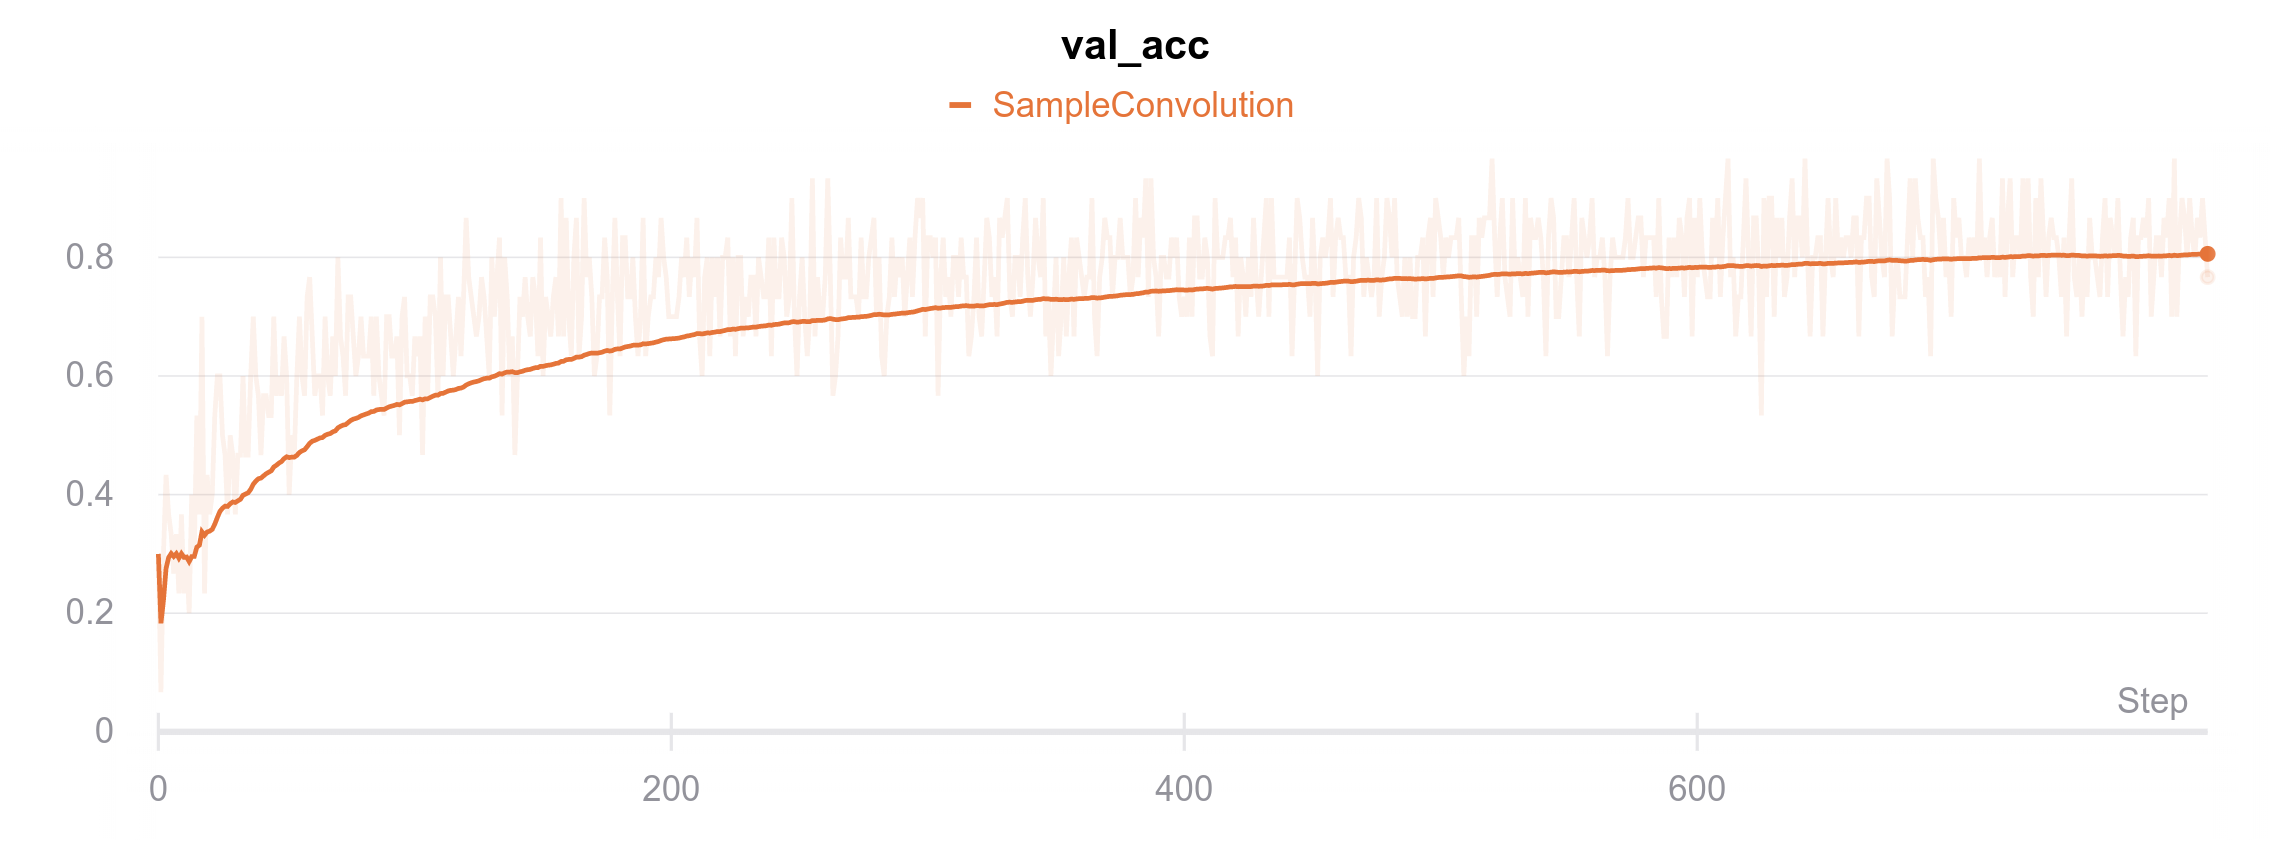
\includegraphics[width=0.7\linewidth]{images/val_acc.png}
                    \end{minipage}
            \end{columns}
	\end{frame}	
	
	\begin{frame}
		\frametitle{Comparison}
    		\begin{figure}[h]
                \center{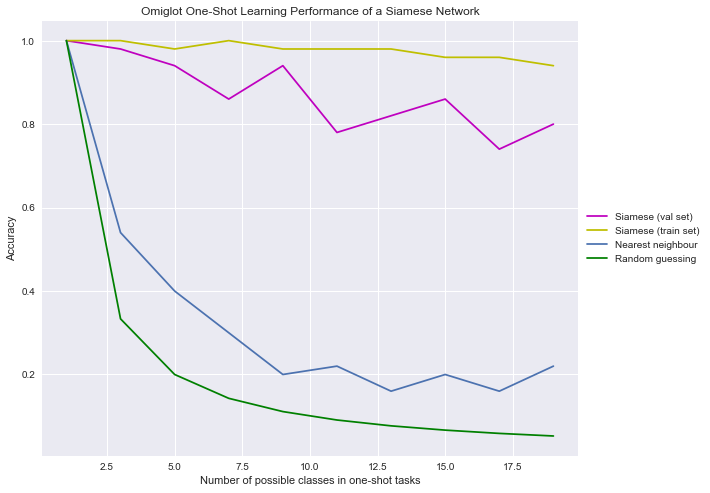
\includegraphics[scale=0.35]{images/comparison.png}}
                \caption{Comparing our approach to nearest neighbour approach}
                \label{fig:image}
            \end{figure}
	\end{frame}		
	
	\begin{frame}
		\frametitle{Conclusions}
		\begin{itemize}
			\item We got about $81$\% average accuracy on evaluation set on 20-way one-shot classification
		\end{itemize}
	\end{frame}
	
	\begin{frame}
		\frametitle{Links}
		\begin{itemize}
			\item Original paper – \url{https://www.cs.cmu.edu/~rsalakhu/papers/oneshot1.pdf}
			\item Implementation – \url{https://github.com/SmirnovAlexander/OneShotLearningSiameseNetworks}
		\end{itemize}
	\end{frame}

\end{document}